\chapter{Theoretische Grundlagen}
\label{sec:grundlagen}
\pagestyle{plain}

\section{Funktionale Programmiersprachen}
\label{sec:funktionaleProgrammiersprache}
%\begin{figure}[htb]
%  \centering  
%  \includegraphics[scale=0.5]{img/starwars.jpg}
%  \caption{Star Wars Logo}
%  \label{fig:starwars}
%\end{figure}
\begin{figure}[ht]
\centering
\begin{lstlisting}[language=JavaScript]
iterative_function(n) {
  sum = 0;
  for(i = 0; i <= n; i++) {
    sum += i;
  }
}
console.log(iterative_function(10)); // => 55
\end{lstlisting}
\caption{Eine iterative Funktion}\label{fig:iterative-function}
\end{figure}
In der Programmierung gibt es zwei Programmierparadigmen, die zur Kategorisierung von Programmiersprachen dienen und sich im Laufe der Zeit entwickelt haben. %„https://de.wikipedia.org/wiki/Programmiersprache#Programmierparadigmen“)
Dabei beschreiben die Paradigmen verschiedene Prinzipien der Programmierung.
Die zugrunde liegenden Kategorien werden häufig als imperative und deklarative Programmierung bezeichnet, in welchen sich jede Programmiersprache einordnen lässt. Jede Kategorie birgt weitere Unterkategorien und dient der Verfeinerung der Prinzipien.
Häufig gehören funktionale Programmiersprachen dem deklarativen Programmierparadigma an. Es ist jedoch nicht ausgeschlossen, dass eine Programmiersprache mehreren Kategorien zugehörig ist und dadurch die Merkmale von mehr als einem Paradigma unterstützt. Zur Gruppe der deklarativen Programmiersprachen zählt man unter anderem Abfragesprachen wie SQL, sowie funktionale Programmiersprachen wie Lisp oder Scheme.
Programmiersprachen der deklarativen Programmierung haben ihren Ursprung in der Mathematik. Programme werden hier als mathematische Funktionen formuliert, die nicht länger beschreiben, was getan werden soll, sondern lediglich vorgeben, welches Ergebnis am Ende erwartet wird.
Bei funktionalen Programmiersprachen ist es üblich, dass eine Variable nach ihrer Initialisierung ihren zugewiesenen Wert für die gesamte Laufzeit des Programmes beibehält und unveränderlich bleibt. Es ist dementsprechend stets nachzuvollziehen, welchen Wert ein Ausdruck besitzt, wodurch insbesondere akademische Anforderungen an ein Programm, wie etwa die Beweisführung, erfüllt werden können. Zusätzlich können auch unendliche Datenstrukturen behandelt werden.
Typischerweise gibt es in funktionalen Programmiersprachen keine Schleifen, da dies bereits eine Verletzung der Unveränderlichkeit von Variablen bedeuten würde, wie klar erkennbar bei der Iteration in Abbildung~\ref{fig:iterative-function} ist. Hier wird bei jedem Durchlauf der Schleife die Variable $i$ inkrementiert und mit dem neuen Wert versehen.

Es ist allerdings auch möglich eine Schleife in einer funktionalen Programmiersprache zu verwirklichen. In Abbildung~\ref{fig:recursive-function} ist die zuvor gezeigte iterative Funktion als rekursive Funktion implementiert worden.
\begin{figure}[hb]
\begin{lstlisting}[language=JavaScript]
recursive_function(n) {
  if (n < 1) return 0
  else return n + recursive_function(n-1);
}
console.log(recursive_function(10)); // => 55
\end{lstlisting}
\caption{Eine rekursive Funktion}\label{fig:recursive-function}
\end{figure}

In beiden Fällen ist das Ergebnis gleich, jedoch besitzt die rekursive Implementierung keinerlei Seiteneffekte. Es wird an keiner Stelle der Wert einer Variable verändert, es werden lediglich Aufrufe mit neuen Werten durchgeführt. Die iterative Implementierung verursacht hingegen zwei Seiteneffekte. Es wird sowohl die Variable $sum$, sowie $i$ bei jedem Schleifendurchlauf überschrieben. Bei der Rekursion hingegen wird  die Funktion $resursive\_function$
mit einem neuen Wert aufgerufen, ohne jemals die ursprüngliche Variable verändert zu haben.
Üblicherweise werden Funktionen in funktionalen Programmiersprachen als Funktionen höherer Ordnung angesehen. Das heißt, dass eine Funktion eine andere Funktion als Argument entgegen nehmen kann, oder eine Funktion als Rückgabewert hat. Diese Art von Funktionen ist bekannt unter dem Begriff $Lambda-Funktion$ oder $anonyme Funktion$. Eine solche Funktion hat entsprechend keinen Namen, sondern kann nur durch einen Verweis aufgerufen werden. Im folgenden Beispiel sehen wir den Aufruf einer anonymen Funktion in Elm:
\begin{equation} \label{eq:solve}
(\backslash x \rightarrow x * 2)\ [ 2, 3, 4 ] \Longrightarrow [4, 6, 8]
\end{equation}
Grundsätzlich wird mit einer solchen Lambda-Funktion ein mathematisches Abbildungsgesetz formuliert. Das mathematische Gegenstück zu Funktion~\ref{eq:solve} ist $x \rightarrow x * 2$ und beschreibt eine Funktion, die einen Eingabeparameter $x$ auf $x*2$ abbildet. Auch Elm gehört dem deklarativen Programmierparadigma an und vereinheitlicht dessen Konzepte.

\section{Grundlagen der Programmiersprache Elm}
\label{sec:Was ist Elm?}

\subsection{Geschichte}
\label{sec:Geschichte}
Elm ist eine funktionale Programmiersprache. Sie wurde im Rahmen der Bachelorarbeit „Elm: Concurrent FRP for Functional GUIs“\\
 (http://Elm-lang.org/papers/concurrent-frp.pdf)
von Evan Czaplicki entwickelt und im April 2012 offiziell veröffentlicht.
Auslöser für die Entwicklung von Elm war für Czaplicki die Schwierigkeit, ein Bild auf einer Webseite sowohl horizontal, als auch vertikal zu zentrieren. Es gab keine für ihn annehmbare, leichte Lösung für dieses Problem, ohne damit weitere Probleme zu schaffen. Unter der Leitfrage „What would web programming look like if we could restart?“ („Wie würde Web-Programmierung aussehen, wenn wir neu starten könnten?“) machte er sich Gedanken, welche Veränderungen an den aktuellen, etablierten Programmiersprachen für die Webentwicklung wünschenswert wären und entwickelte den ersten Prototypen von Elm.

\subsection{Konzept}
\label{sec:Konzept}
\begin{figure}[h]
	\centering  
	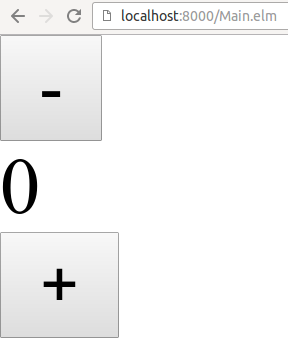
\includegraphics[scale=0.5]{img/counter.png}
	\caption{Ein simpler Zähler auf einer Webseite}\label{fig:counter}
\end{figure}
\noindent Elm verfolgt eine ganz eigene Implementierung des Model-View-Controller Paradigmas. Hier wird es \ac{MVU} genannt. Anhand des Beispiels in Abbildung~\ref{fig:counter} lässt sich das Muster in drei grundlegende Stationen unterteilen und erklären.

Die Abbildung~\ref{fig:counter} zeigt einen simplen Zähler der über zwei Knöpfe inkrementiert und dekrementiert werden kann. Der aktuelle Stand des Zählers wird zwischen den Knöpfen angezeigt und kann sowohl negative, als auch positive Werte annehmen.
Der angezeigte Zählerwert ist das sogenannte $Model$ und zeigt den aktuellen Status der Applikation an. Interagiert ein Nutzer nun mit einem der beiden Knöpfe um den Zähler zu erhöhen oder zu reduzieren, wird diese Aktion an die sogenannte $Update$-Funktion weitergegeben. Zusätzlich zur auszuführenden $Aktion$, bekommt diese Funktion auch noch das aktuelle $Model$, sprich den momentanen Zählerwert übergeben.
Die $Update$-Funktion nimmt sämtliche Einwirkungen durch den Nutzer von außen entgegen und wendet diese Aktionen auf das aktuelle $Model$ an. Das bedeutet in diesem konkreten Fall, dass das $Model$ erhöht oder reduziert wird. Dabei wird jedoch nicht das $Model$ direkt verändert, sondern ein neues $Model$ mit den geänderten Werten wird zurückgegeben, da sonst ein Seiteneffekt die Folge wäre. Damit dieser Vorgang zügig vonstatten geht, nutzt Elm persistente Datenstrukturen, womit nur die tatsächlich geänderten Attribute eines Models im neuen $Model$ gesetzt werden, die unveränderten Attribute hingegen werden übernommen.
Das Ergebnis der Update-Funktion wird weitergereicht an die $View$-Funktion. Sie beschreibt das Aussehen der Website, soll heißen wie das $Model$ dargestellt wird. Elm nutzt ein virtuelles \ac{DOM}, wodurch nur tatsächliche Änderungen im Browser angezeigt werden, anstatt dauerhaft das komplette \ac{DOM} stetig zu aktualisieren. Das \ac{DOM} beschreibt die Schnittstelle zum Datenzugriff auf das Objektmodell eines \ac{HTML}-Dokumentes.
Der Datenfluss in Elm wird noch einmal in Abbildung~\ref{fig:elm-model-view-update-concept} visualisiert.
\begin{figure}[h]
  \centering  
  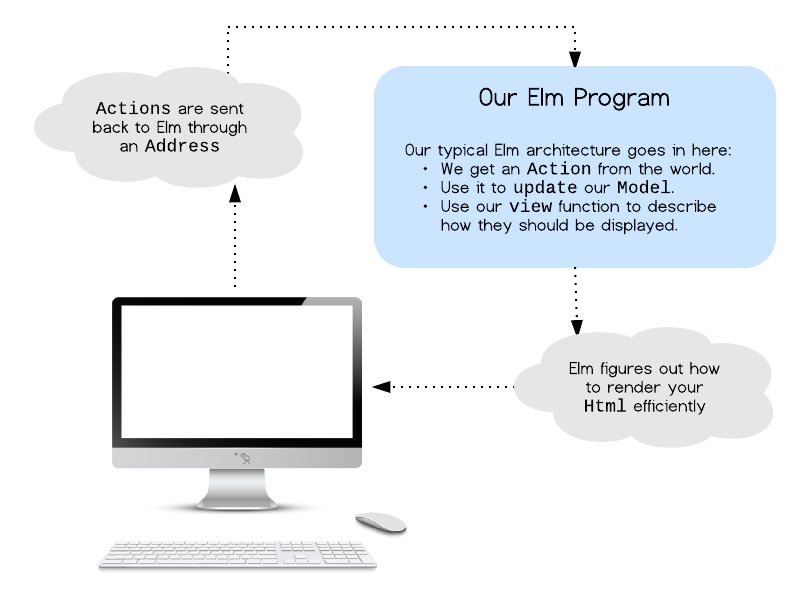
\includegraphics[scale=1]{img/elm-model-view-update-concept.png}
  \caption{Das Model-View-Update Konzept von Elm}\label{fig:elm-model-view-update-concept}
\end{figure}

\subsection{Umsetzung}
\label{sec:Umsetzung}
Der vom Programmierer verfasste Programmcode wird vor der endgültigen Nutzung zu \ac{JS}, \ac{HTML} und \ac{CSS} kompiliert und in die Webseiten integriert. Entsprechend fungiert in Elm verfasster Code im Endeffekt wie natives \ac{JS}, nutzt allerdings noch einige weitere vertiefende Konzepte, um viele Problematiken von \ac{JS} zu umgehen und auszumerzen.
Unter anderem verspricht Elm, dass generierter Code keinerlei Laufzeitfehler (http://elm-lang.org/) erzeugt. Sämtliche Fehlerquellen werden vom Compiler zuvor erkannt, abgefangen und an den Programmierer weitergeleitet, um sie zu beheben. Damit dies funktioniert, implementiert Elm mehrere Konzepte des deklarativen Programmierparadigmas.

\subsubsection{Keine Seiteneffekte}
\label{sec:Keine Seiteneffekte}
Ein Seiteneffekt beschreibt die mehrmalige Zuweisung einer Variable mit einem Wert. In Elm ist das allerdings nicht möglich. Sämtliche Variablen sind unveränderlich und können nur einmalig mit einem Wert initiiert werden. Danach bleibt diese Variable bis zum Ende der Laufzeit unverändert. Wie bereits beschrieben gibt es in Elm das Model, welches die Informationen über den Status der Applikation darstellt. Beschreibt das $Model$ beispielsweise den aktuellen Stand eines Zählers und wird dieser erhöht, muss auch das Model, um aktuell zu bleiben, verändert werden. Hier käme es zu einem Seiteneffekt. Realisiert wird diese Veränderung dadurch, dass ein neues $Model$ mit den gleichbleibenden Daten, sowie dem zu ändernden, aktualisierten Wert erstellt wird. Da ein neues $Model$ erstellt wurde, gibt es nun keinen Seiteneffekt mehr. Das vorherige $Model$ wird schlichtweg verworfen und ersetzt.
Das Konzept der unveränderbaren Werte wurde aus der Mathematik übernommen.  Um Funktionen und ihre Korrektheit garantieren zu können, wird dort dasselbe Prinzip der unveränderlichen Variablen angewandt. Betrachtet man beispielsweise den folgenden Code, so fällt auf, dass die Schreibweise lediglich in den meisten imperativen Programmiersprachen sinnvoll ist, allerdings einen Seiteneffekt darstellt.
\begin{equation} \label{eq:imperative_equation}
x = x + 1
\end{equation}
In einer imperativen Programmiersprache wird der Ausdruck~\ref{eq:imperative_equation} den aktuellen Wert in $x$ auslesen, um $1$ inkrementieren und das Ergebnis der Operation in die Variable $x$ schreiben.
Mathematisch betrachtet ist diese Aussage jedoch schlichtweg falsch, denn es existiert kein $x$, welches diese Aussage wahr werden lässt:
\begin{equation} \label{eq:mathematical_equation}
x=x+1 \leftrightarrow 0=1
\end{equation}
Die meisten imperativen Programmiersprachen nutzen das rechtsassoziative Gleichheitszeichen als Zuweisung, während in der Mathematik das Gleichheitszeichen als Vergleichsoperator angesehen wird.
Die eigentliche Bedeutung des Ausdrucks~\ref{eq:imperative_equation} ist mathematisch ausgedrückt:
\begin{equation} \label{eq:true_equation}
x_1:= x_0 + 1
\end{equation}
Es ist klar erkennbar, dass $x_1$ und $x_0$ nicht dieselbe Variable sind wodurch die Aussage nun als wahr eingestuft werden kann. Das beschriebene Konzept wird referentielle Transparenz genannt und beschreibt die Kontinuität des Wertes einer Variable.
Des Weiteren basieren Funktionen in Elm auf dem Konzept von reinen Funktionen($pure functions$). Das bedeutet, dass eine Funktion stets das gleiche Ergebnisse liefert, insofern auch die Eingabeparameter gleich bleiben, unabhängig vom Zeitpunkt der Ausführung. Beispiele für eine reine Funktion sind $sin(x)$ oder $add(x, y)$. Sie berechnen immer dieselben Werte, völlig unabhängig davon, wie oft oder zu welchem Zeitpunkt sie ausgeführt werden. Ein beliebtes Gegenspiel ist die $random()$ Funktion, die einen (semi-)zufälligen Wert zurückliefert und somit als eine unreine Funktion gilt. Doch auch diese Funktion kann zu einer reinen Funktion gemacht werden, wenn man sie einen Wert abhängig von einem Übergabeparameter berechnen lässt wie beispielsweise $random(seed)$.

\subsubsection{Elm-Compiler}
\label{sec:Elm-Compiler}
Laufzeitfehler sollen mit Elm in Vergessenheit geraten. Dafür soll der integrierte Compiler sorgen. Die Fehlermeldungen des Compilers sind sehr strikt und deuten exakt auf die Programmzeile die für den jeweiligen Fehler verantwortlich ist. Bei der herkömmlichen Entwicklung eines Frontends mit \ac{JS} trifft man häufig auf den Wert $undefined$. Dieser Wert beschreibt, dass die dazugehörige Variable noch nicht initialisiert wurde und somit keine nutzbaren Daten enthält. Trifft man nun auf diesen Wert und versucht eine andere Funktion darauf auszuführen, so kann das geschriebene Programm entsprechend abstürzen. Der Elm Compiler überprüft den Programmcode nach exakt diesen Situation beziehungsweise analysiert, ob Variablen und Funktionen vorab initialisiert wurden, welche Parameter die einzelnen Funktionen erwarten und ob die Rückgabeparameter dem Typen entsprechen, den die anderen Funktionen erwarten. Befolgt man die Anweisungen des Compilers, soll das in einem stark strukturierten, lesbaren und funktionieren Code münden.
Dem Programmierer werden weniger Möglichkeiten gegeben, bestimmte Ziele zu erreichen, doch dadurch soll auf lange Sicht einheitlicher, lesbarer und besser zu wartender Code erzeugt werden. Passend dazu gibt es bereits viele Erweiterungen für gängige Editoren wie Sublime Text und Atom, welche beim Speichern des Projektes den Code entsprechend des Style Guides strukturieren und formatieren. So kann einerseits die Lesbarkeit des Codes vereinheitlicht, andererseits die Fehlerquellen in Form von Einrückungsfehlern oder vergessenen Kommas o.ä. verringert werden.

\subsubsection{Statische Typisierung}
\label{sec:Statische Typisierung}
Anders als bei nativem \ac{JS}, gibt es in Elm keine dynamische Typisierung. Das bedeutet, dass sowohl die Typen einer Variable, als auch die Rückgabewerte von Funktionen bereits bei der Kompilierung bekannt sein müssen. Natives \ac{JS} erlaubt es, dass die Typen von Variablen erst zur Laufzeit überprüft werden und sich zusätzlich in dieser Zeit ändern können. So ist der Quellcode in Abbildung~\ref{fig:dynamische-typisierung} konform in \ac{JS}.
\begin{figure}[ht]
	\centering
		\begin{lstlisting}[language=JavaScript]
		var i = 1;
		i = "Test";
		\end{lstlisting}
\caption{Beispiel der dynamischen Typisierung}\label{fig:dynamische-typisierung}
\end{figure}
Der Typ der Variable $i$ wurde in der Abbildung~\ref{fig:dynamische-typisierung} während der Laufzeit von $number$ zu $string$ geändert. Da Elm stark typisiert ist, gibt es keine Möglichkeit, dass eine Funktion verschiedene Datentypen zurück gibt oder eine Variable mehrere Typen während der Laufzeit annimmt.

\subsubsection{Modularität}
\label{sec:Modularität}
Um geschriebenen Code auch in Zukunft wartbarer zu machen, ist Elm modular aufgebaut und leicht erweiterbar. Es ist denkbar einfach vorhandenen Code zu importieren. Die importierten Module verstehen sich als gekapselt, wodurch sie in keiner Weise mit dem bereits verfügbaren Code kollidieren können.


\subsubsection{Performanz}
\label{sec:Performanz}
\begin{figure}[hb]
  \centering  
  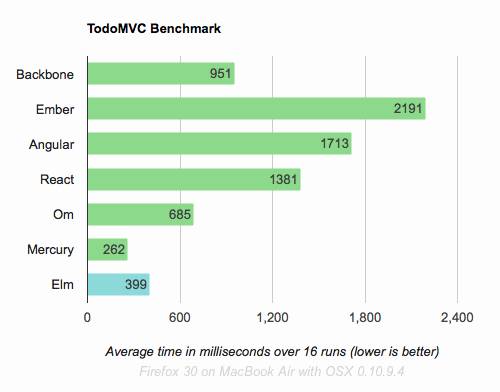
\includegraphics[scale=0.6]{img/virtual-dom.png}
  \caption{Performanz von Elm im Vergleich zu anderen Web-Frameworks. \cite{elm-performance}}\label{fig:performance}
\end{figure}
Obwohl Daten nicht verändert, sondern lediglich als neuer aktualisierter Datensatz betrachtet werden und einzelne Funktionen stark ausgelagert werden können, leidet die Performanz nicht darunter. Laut Abbildung~\ref{fig:performance} überzeugt Elm mit einer sehr guten Geschwindigkeit. Möglich wird das durch die Verwendung eines virtuellen \ac{DOM}.
Dabei wird das echte \ac{DOM} bei jedem „Frame“ in eine abstrakte Version kopiert. Auf diese abstrakte Version werden die Änderungen angewandt. Zunächst klingt diese Vorgehensweise sehr langsam und aufwändig, doch um die Geschwindigkeit zu gewährleisten wird das aktuelle abstrakte \ac{DOM} mit dem neuen, veränderten \ac{DOM} verglichen und nach Unterschieden gesucht. Jede Unterschiedlichkeit wird daraufhin zu einer Liste hinzugefügt, in der sämtliche Änderungen festgehalten werden. Anschließend wird diese Liste an den Browser zurückgegeben, so dass alle Änderungen für den Nutzer sichtbar gemacht werden können. Daraus resultiert, dass nur noch die tatsächlich neuen Elemente im \ac{DOM} des Nutzers aktualisiert werden müssen. Dieser zu verändernde Teil stellt nur einen Bruchteil des kompletten \ac{DOM} dar. Man kann dadurch von einer immensen Effizienzsteigerung ausgehen.


\subsubsection{Interoperabilität}
\label{sec:Interoperabilität}
Es wäre sehr aufwendig die gängigsten JavaScript-Bibliotheken und -Frameworks wie jQuery oder AngularJS komplett zu verwerfen und erneut mit Elm zu realisieren respektive neu zu programmieren. Glücklicherweise bietet Elm eine ausgereifte Interoperabilität, wodurch alle Garantien der deklarativen Programmierung übernommen werden können, selbst wenn die externen Bibliotheken diese nicht gewährleisten.
Die genannten externen Bibliotheken sind zum Großteil nicht deklarativ programmiert, weswegen normalerweise keinerlei Garantien seitens Elm gemacht werden können. Jedoch ist Elm von den externen Bibliotheken isoliert und kommuniziert nur über sogenannte Ports mit JavaScript. Die Kommunikation durch die Ports funktioniert in beide Richtungen, womit sämtliche Daten bei Bedarf ausgetauscht werden können. Da in Elm wie bekannt vorab die Typen der Eingabeparameter und Rückgabewerte spezifiziert werden müssen, werden die Garantien weiterhin gewahrt.

\subsubsection{Debugger}
\label{sec:Debugger}
Nicht nur die detaillierten Fehlermeldungen des Compilers sind ein großer Pluspunkt von Elm, sondern auch der mitgelieferte und einfach zu bedienende Debugger. Anders als bei anderen Programmiersprachen zeigt der Debugger nicht nur einen einfachen Stacktrace mit den letzten Rücksprungadressen an. Vielmehr ermöglicht es der Debugger in Elm die Zeit zurückzudrehen. In gängigen Debuggern ist es nicht einfach, ein bestimmtes Verhalten, das möglicherweise zum Absturz des Programms geführt hat, zu reproduzieren. Um den Fehler erneut zu erhalten und dadurch ein Verständnis des Fehlers aufzubauen ist es oft notwendig den genauen Hergang und Ablauf manuell nachzuahmen. Der Elm Debugger hingegen speichert den Status einer jeden Variable zu jedem Zeitpunkt und zeichnet außerdem die Wechsel auf. Aufgrund dessen ist es sehr einfach möglich mit Hilfe eines Sliders auf der Website die Zeit buchstäblich zurückzudrehen und den vorherigen Status wieder aufzurufen. Weiterhin besteht die Möglichkeit sämtliche Daten zu diesem Zeitpunkt zu betrachten und live zu verändern. Dadurch wird nicht nur der aktuell begutachtete Status verändert und der Effekt zeitgleich auf dem Bildschirm angezeigt, sondern auch alle folgenden Status mitsamt den Daten werden entsprechend aktualisiert. Evan Czaplicki hat dahingehend ein Video angefertigt, dass den Vorgang sehr detailliert beschreibt (LINK). Alternativ kann die Abbildung XY betrachtet werden, die einen Zeitstrahl mit Werten, sowie die Möglichkeiten die sich durch den Debugger ergeben, aufzeigt.


\subsubsection{Praktische Anwendungsgebiete}
\label{sec:Praktische Anwendungsgebiete}
Elm ist noch recht neu und befindet sich im ständigen Wandel. Für viele Entwickler ist Elm entsprechend noch keine wirkliche Alternative zu ihren gegenwärtig genutzten Frameworks, obgleich die Entwicklung mit den gängigen Werkzeugen oftmals steinig ist. Nur wenige Unternehmen nutzen derzeit Elm in ihrem Produktionsumfeld. Die wohl derzeit größten Nutzer sind NoRedInk, Prezi und CircuitHub. Alle Betriebe überführen Stück für Stück bereits bestehende Teile ihres Frontends zu Elm. NoRedInk gibt an, dass der überführte Elm-Code in den letzten acht Monaten keinerlei Laufzeitfehler erzeugt hat, anders als die vorherige Implementierung\\ (https://www.youtube.com/watch?v=zBHB9i8e3Kc). Dennoch wird es wohl noch eine Weile dauern, bis sich mehr Firmen der Vorstellung hingeben ihr lauffähiges System in die vielversprechende Programmiersprache Elm zu portieren, nicht zuletzt, weil sie sich noch in einem sehr frühen Stadium befindet und somit noch nicht völlig ausgereift ist.
Es existiert jedoch bereits eine Vielzahl an Projekten die mit Elm verwirklicht wurden. Dabei sind viele dieser Projekte kleinere Retro-Spiele, die über den Browser gespielt werden können \footnote{\cite[vgl.]{builtwithelm}}. Dazu gehört unter anderem Tetris, Pong und Space Invaders. Weiterhin bietet Elm sehr einfache Möglichkeiten Formen wie Kreise, Vierecke, Hexagone und vieles mehr zu erzeugen, ohne großartig in die Mathematik einzusteigen.\\
Dieser Einblick zeigt bereits, dass Elm in vielerlei Hinsicht Besserung für die Entwicklung von Webapplikationen verspricht. Doch wie praktikabel sind diese Versprechungen? Ist die Programmiersprache effizient und intuitiv, oder durch ihr noch frühes Entwicklungsstadium unausgereift?
„The best functional programming in your browser“ - Diese Aussage wird anhand verschiedener Bewertungskriterien überprüft.
Im Zuge dessen wird eine Webseite mit kleineren Modulen in Elm erzeugt. Die fertige Webseite respektive der erzeugte Quellcode wird anhand der zuvor erstellten Bewertungskriterien ausgewertet. Auch die Beobachtungen während der Entwicklung, wie etwa unvorhergesehene Probleme, gehen mit in die Wertung ein.

\subsection{Einführung in die Elm-Architektur}
\label{sec:elm-architektur}
TODO: Evtl. Absatz \nameref{sec:Praktische Anwendungsgebiete} hier rein mergen und abändern?
... Um eine Programmiersprache jedoch anzuwenden, ist es notwendig zuvor die Architektur kennenzulernen. Dieses Kapitel soll eine Einführung in die Programmiersprache Elm darstellen und die grundlegenden Funktionen näher bringen.

\subsubsection{Basisdatentypen}
\label{sec:Basisdatentypen}
Elm hat nur eine geringe Anzahl an Basisdatentypen, mithilfe derer sämtliche weiterführende Konstrukte abgeleitet werden können:
\begin{itemize}
	\item 42 : Number
	\item True : Bool
	\item 'a' : Char
	\item {[1, 2, 3] : List}
\end{itemize}
Durch die Kombination dieser Basisdatentypen können andere Datentypen wie $Strings$, $Integer$ oder $Floats$ erzeugt werden.

\subsubsection{Union Types}
\label{sec:Union-Types}

\subsubsection{Objekte}
\label{sec:Objekte}
Auch in Elm ist es notwendig Informationen während der Laufzeit zwischen zu speichern und nicht direkt zu verlieren. In anderen Programmiersprachen gibt es dafür sogenannte $Objekte$ oder $Variablen$.

\subsubsection{Funktionen}
\label{sec:Funktionen}
\begin{figure}[h]
\begin{lstlisting}[language=JavaScript]
add : Int -> Int -> Int
add a b =
  a + b

add 3 4   -> 7
\end{lstlisting}
\caption{Eine Funktion in Elm}\label{fig:elm-function}
\end{figure}
Um in irgendeiner Art und Weise eine Interaktion mit den erstellten $Records$ zu vollziehen, benötigt der Entwickler auch in Elm eine Funktionen. Solch ein Programmkonstrukt wird mittels eines Funktionsnamen und dem Gleichheitszeichen realisiert.

Abbildung~\ref{fig:elm-function} zeigt, wie eine simple Addition zweier Integer-Werte umgesetzt wird. Die Buchstaben $a$ und $b$ deuten an, dass die Funktion $add$ zwei Parameter erwartet. Der gesamte Inhalt nach dem Gleichheitszeichen ist der sogenannte Rumpf einer Funktion und beschreibt den anzuwendenden Algorithmus. Der Funktionsaufruf ist in Zeile 5 sichtbar. Auffällig ist, dass eine Funktion nie explizit einen Wert zurück gibt, wie es in anderen Programmiersprachen wie \ac{JS} oder C++ meist durch den Befehl $return$ geschieht. Elm gibt implizit die letzte ausführbare Zeile als Rückgabewert zurück. Der beispielhafte Aufruf der Funktion $add$ in Zeile 5 hätte dementsprechend $7$ als Ergebnis. Des Weiteren ist erkennbar, dass Elm ohne die Nutzung von Kommata oder Klammern auskommt. Klammern werden erst notwendig, wenn mehrere Funktionen geschachtelt ablaufen sollen und eine Auswertung der Befehle von links nach rechts nicht ausreicht.

\subsubsection{Signaturen}
\label{sec:Signaturen}
Zeile 1 in Abbildung~\ref{fig:elm-function} zeigt den Aufbau einer Signatur. Solch eine Signatur beschreibt die Funktion. Dabei sind Informationen über die Anzahl und der jeweilige Typ der Übergabeparameter, sowie der Typ des Rückgabewertes enthalten. Anhand der Abbildung~\ref{fig:elm-function} lässt sich erkennen, dass die $add$-Funktion zwei Parameter vom Typ $Int$ erwartet und letzten Endes ein Ergebnis des Typ $Int$ liefert. Fehlt einer Funktion die Signatur, wird der $elm-compiler$ eine Warnung ausgeben und zusätzlich eine passende, jedoch teilweise allgemeinere Signatur ausgeben. Würde die Funktion in Abbildung~\ref{fig:elm-function} keine Signatur enthalten, würde der $elm-compiler$ die Signatur $add : Number -> Number -> Number$ vorschlagen. Da ein $Int$ nur eine Spezifizierung des Basisdatentypen $Number$ darstellt, ist das nicht verwunderlich. Der $elm-compiler$ nutzt implizit die eigens erarbeiteten Signaturen bei der Überprüfung des Quellcodes, sollte der Entwickler keine Signatur angegebenen haben.

\subsubsection{Module}
\label{sec:Module}
\begin{figure}[h]
\begin{lstlisting}[language=JavaScript]
module MyModule exposing(..)
module MyModule exposing (add, anotherMethod)
\end{lstlisting}
\caption{Mögliche Deklarationen eines Elm-Moduls}\label{fig:elm-module}
\end{figure}
Oftmals ist es sinnvoll Quellcode der sich nur auf eine Problemlösung bezieht zu gruppieren. Auch in Elm ist es möglich Code auszulagern in sogenannte $Module$. Sie beschreiben eine Art Container, in dem der Code isoliert von den anderen Projektteilen betrachtet werden kann. Um ein $Modul$ in Elm zu erstellen, muss eine neue Datei vom Typ $elm$ erzeugt werden. Abbildung~\ref{fig:elm-module} zeigt zwei Beispiele, wie eine Quelldatei als Modul deklariert werden kann. Zeile $1$ gibt dabei sämtliche Funktionen die im Modul beinhaltet sind nach außen weiter, sobald das Modul importiert wird. Dies sollte nur gemacht werden, wenn das Modul sich um eine Art Bibliothek handelt, in der sämtliche Funktionen verfügbar gemacht werden sollen. In Zeile $2$ hingegen wird ersichtlich, wie nur ausgewählte Funktionen nach außen sichtbar gemacht werden. In diesem Falle sind die Funktionen $add$ und $anotherMethod$ nutzbar.

- Quellcode wird unübersichtlich
- Funktionen haben nichts mehr miteinander zu tun (Gruppierung sinnlos...)
- Funktionen können in Module ausgelagert werden, die sich gezielt mit einem Problem auseinander setzen / eine Problemlösung anstreben.
- Module können importiert werden.
- Module können bestimmen, welche Informationen an die 'Außenwelt' freigegeben werden.


\subsubsection{Online-IDE}
\label{sec:Online-IDE}
\begin{figure}[h]
	\centering
	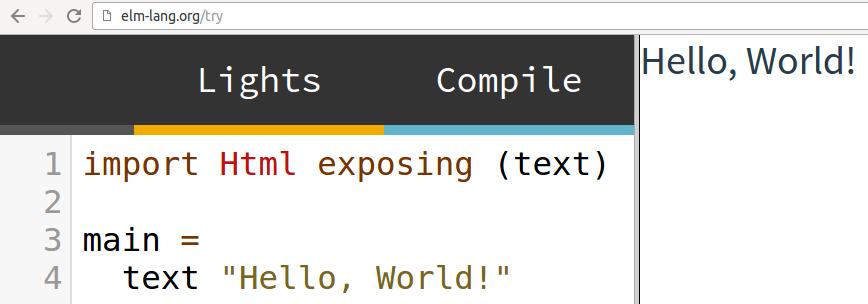
\includegraphics[scale=0.4]{img/elm-try.png}
	\caption{Die Online-\ac{IDE} von Elm}\label{fig:elm-try}
\end{figure}
Möchte man beginnen mit Elm zu programmieren, so ist es nicht notwendig sämtliche Tools auf dem lokalen Gerät zu installieren. Vielmehr haben die Entwickler von Elm eine Online-\ac{IDE} erstellt, mit der sofort entwickelt werden kann. Abbildung~\ref{fig:elm-try} zeigt diese \ac{IDE} mit einem typischen $Hello-World$ Beispiel. Auf der linken Seite ist eigentliche \ac{IDE} erkennbar, während die rechte Seite das Ergebnis nach dem Kompiliervorgang ausgibt. Sollte es einen Fehler während des kompilierens geben, wird die entsprechende Fehlermeldung des $elm-compiler$ dort ausgegeben. Mit Hilfe der Schaltfläche $Lights$ können zum Einen die Farben der \ac{IDE} invertiert werden, während der Knopf $Compile$ den geschriebenen Quellcode kompiliert und ausführt. Kleinere Projekte kön	nen entsprechend bequem mit diesem Tool realisiert werden. Die \ac{IDE} bietet einen schnellen Einstieg in die Programmiersprache.

